\chapter{Testing and Quality Assurance}
\label{ch:testing}

\begin{quote}
\emph{``Testing shows the presence, not the absence, of bugs.''} --- Dijkstra. QA is therefore a layered net---unit, integration, and system tests plus process discipline---so no single hole lets a critical defect through.
\end{quote}

\noindent\fbox{\parbox{\dimexpr\linewidth-2\fboxsep-2\fboxrule}{%
\textbf{From zero: no prior testing course assumed.} We define \emph{test case}, \emph{oracle}, \emph{coverage}, \emph{mock}, and \emph{quality assurance} from first principles with intuition before formalism. We assume working code (Ch.~5) and requirements to verify against (Ch.~2). No statistics beyond basic counting is needed.}}

\vspace{0.4em}

\section*{Learning Outcomes}
After this chapter you will be able to:
\begin{enumerate}[label=(L\arabic*)]
    \item design unit tests with boundary and partition techniques and interpret coverage honestly;
    \item write integration and system tests that exercise contracts between layers and with external services;
    \item apply test-driven development (TDD) and distinguish its benefits from testing after the fact;
    \item build a QA plan with reviews, static analysis, and acceptance criteria linked to the traceability matrix;
    \item reason about defect cost curves and risk-based test prioritisation under semester constraints.
\end{enumerate}

% ============================================================
\section{Unit Testing: The First Net}
\label{sec:unit-testing}

\textbf{Intuition.} A unit is the smallest testable piece (a function, class, or module) isolated from its collaborators by \emph{test doubles}. If every brick is sound, the wall is more likely to stand---but unit tests alone do not prove the wall is straight.

\begin{definition}[Test Case and Oracle]
A \emph{test case} is a triple $(\text{input}, \text{precondition}, \text{expected output})$. The \emph{oracle} is the mechanism that decides pass/fail---often an \texttt{assert} against the expected value or a property.
\end{definition}

\textbf{Design techniques.} (i)~\emph{Equivalence partitioning:} split inputs into classes that should behave identically and test one per class. (ii)~\emph{Boundary value analysis:} test edges ($0,1,\max,\max+1$) where off-by-one and fencepost bugs cluster. (iii)~\emph{Decision tables / pairwise:} for combinational logic, cover meaningful combinations without exhaustive explosion. A good unit suite is \emph{FAST}: Fast, Automated, Small scope, Trustworthy.

\begin{lstlisting}[language=Python,caption={Unit tests with partitions, boundaries, and mocking. Each test name states the scenario and expected outcome.},label={lst:unit-test}]
import pytest
from unittest.mock import Mock
from app.pricing import discount

# partitioning: age -> rate; boundaries at 0,12,13,59,60,120
@pytest.mark.parametrize("age,expected", [
    (12, 0.50),   # boundary: child upper edge
    (13, 0.25),   # boundary: teen lower edge
    (59, 0.25),   # boundary: teen upper edge
    (60, 0.00),   # boundary: adult lower edge
])
def test_discount_boundaries(age, expected):
    assert discount(age) == pytest.approx(expected)

def test_discount_uses_repo_via_mock():
    repo = Mock()
    repo.get_user.return_value.age = 10
    # SUT calls repo; mock isolates the unit from the database
    assert discount(repo.get_user("u1").age) == 0.50
    repo.get_user.assert_called_once_with("u1")

def test_discount_invalid_age_raises():
    with pytest.raises(ValueError):
        discount(-1)
\end{lstlisting}

\textbf{Coverage (with caveats).} Line/branch coverage measures what code \emph{ran}, not what was \emph{checked}. 100\% coverage with weak oracles still misses bugs; 70\% with strong oracles often beats 95\% with flabby ones. Use coverage to find \emph{untested} code, not to prove correctness. Enforce a floor (e.g., 70\%) in CI, but require meaningful assertions to count.

% ============================================================
\section{Integration and System Testing}
\label{sec:integration-system}

Unit tests mock collaborators; \emph{integration tests} restore them to verify contracts. Test the seams: controller$\leftrightarrow$service, service$\leftrightarrow$repository, and app$\leftrightarrow$external API (with a sandbox or recorded fixture, not live production).

\begin{figure}[h]
\centering
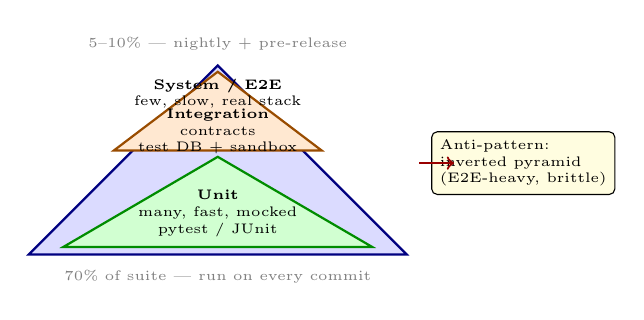
\begin{tikzpicture}[scale=0.80, every node/.style={font=\scriptsize}]
  % pyramid
  \fill[blue!14,draw=blue!50!black,thick] (0,0) -- (6.0,0) -- (3.0,3.0) -- cycle;
  % layers
  \fill[green!18,draw=green!55!black,thick] (0.55,0.12) -- (5.45,0.12) -- (3.0,1.55) -- cycle;
  \fill[orange!18,draw=orange!60!black,thick] (1.35,1.65) -- (4.65,1.65) -- (3.0,2.90) -- cycle;
  % labels
  \node[align=center,font=\tiny] at (3.0,0.65) {\textbf{Unit}\\{\tiny many, fast, mocked}\\{\tiny pytest / JUnit}};
  \node[align=center,font=\tiny] at (3.0,1.95) {\textbf{Integration}\\{\tiny contracts}\\{\tiny test DB + sandbox}};
  \node[align=center,font=\tiny] at (3.0,2.55) {\textbf{System / E2E}\\{\tiny few, slow, real stack}};
  % counts
  \node[font=\tiny,gray] at (3.0,-0.35) {70\% of suite --- run on every commit};
  \node[font=\tiny,gray] at (3.0,3.35) {5--10\% --- nightly + pre-release};
  % side annotation
  \node[draw,fill=yellow!12,rounded corners=2pt,font=\tiny,align=left,inner sep=3pt] at (7.85,1.45) {Anti-pattern:\\inverted pyramid\\(E2E-heavy, brittle)};
  \draw[->,thick,red!60!black] (6.2,1.45) -- (6.75,1.45);
\end{tikzpicture}
\caption{Test pyramid: many fast unit tests at the base, fewer integration tests in the middle, a thin cap of slow end-to-end system tests. Colour darkens with integration cost.}
\label{fig:test-pyramid}
\end{figure}

\emph{System / E2E tests} exercise the whole stack as a user would: Selenium/Playwright for web, or \texttt{pytest} against a test deployment with a real (seeded) database. Keep E2E thin: they are slow, flaky, and expensive to maintain. One happy-path plus a few critical error flows per feature suffices at capstone scale.

\textbf{Mocks, stubs, fakes, and contracts.} A \emph{mock} verifies interactions, a \emph{stub} returns canned data, a \emph{fake} is a lightweight real implementation (in-memory DB). For external services, record/replay (VCR.py) or a contract test that asserts your assumption about the provider's API still holds after their update.

\begin{figure}[h]
\centering
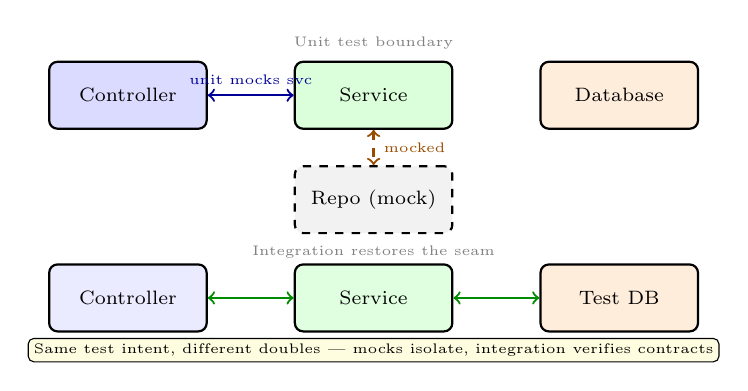
\begin{tikzpicture}[scale=0.78, every node/.style={font=\scriptsize},
  box/.style={draw,thick,rounded corners=3pt,minimum width=2.0cm,minimum height=0.85cm,align=center},
  mock/.style={draw,thick,dashed,rounded corners=3pt,minimum width=2.0cm,minimum height=0.85cm,align=center,fill=gray!10}]
  \node[box,fill=blue!14] (ctrl) at (0,0) {Controller};
  \node[box,fill=green!14] (svc) at (4.0,0) {Service};
  \node[mock] (repo) at (4.0,-1.7) {Repo (mock)};
  \node[box,fill=orange!14] (db) at (8.0,0) {Database};
  \draw[<->,thick,blue!60!black] (ctrl) -- (svc) node[midway,above,font=\tiny] {unit mocks svc};
  \draw[<->,thick,dashed,orange!60!black] (svc) -- (repo) node[midway,right,font=\tiny] {mocked};
  \node[font=\tiny,gray] at (4.0,0.85) {Unit test boundary};
  % integration row
  \node[box,fill=blue!8] (c2) at (0,-3.3) {Controller};
  \node[box,fill=green!12] (s2) at (4.0,-3.3) {Service};
  \node[box,fill=orange!14] (r2) at (8.0,-3.3) {Test DB};
  \draw[<->,thick,green!55!black] (c2) -- (s2);
  \draw[<->,thick,green!55!black] (s2) -- (r2);
  \node[font=\tiny,gray] at (4.0,-2.55) {Integration restores the seam};
  \node[font=\tiny,fill=yellow!12,draw,rounded corners=2pt,inner sep=2pt] at (4.0,-4.15) {Same test intent, different doubles --- mocks isolate, integration verifies contracts};
\end{tikzpicture}
\caption{Unit vs.\ integration boundary: unit tests replace the repository with a mock; integration tests wire the real (test) database to verify the contract. Mocks tell you \emph{you called it right}; integration tells you \emph{it did the right thing}.}
\label{fig:unit-vs-integration}
\end{figure}

% ============================================================
\section{Test-Driven Development and QA Process}
\label{sec:qa-process}

\emph{Test-Driven Development} (TDD) inverts the order: Red (write a failing test) $\to$ Green (minimal code to pass) $\to$ Refactor. Benefits: forces testability, yields a live specification, and makes regression safe---but it suits well-specified logic more than exploratory UI. Use TDD for pricing, validation, and API contracts; prototype UI first, then pin it with approval tests.

\emph{Quality assurance} is wider than testing:

\begin{itemize}
    \item \textbf{Reviews:} peer review every PR; checklists beat memory (correctness, edge cases, tests, naming, traceability to Req ID).
    \item \textbf{Static analysis:} linters, type checkers (\texttt{mypy}, \texttt{tsc}), and security scanners run in CI---they catch the class of bugs tests miss.
    \item \textbf{Acceptance criteria:} every story's Gherkin scenario (Ch.~2) is an executable acceptance test; link \texttt{US-07} $\to$ test $\to$ demo.
\end{itemize}

Risk-based prioritisation: order tests by (likelihood of defect $\times$ impact if shipped). Payment and authentication are high-risk; an about-page typo is not. Under time pressure, protect the red cells of the risk matrix (Ch.~4).

\begin{figure}[h]
\centering
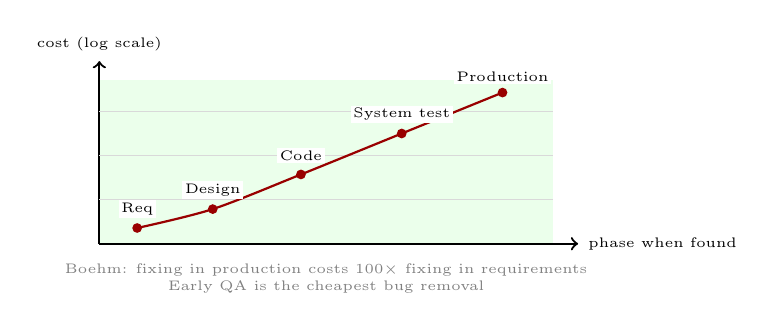
\begin{tikzpicture}[scale=0.80, every node/.style={font=\scriptsize}]
  % cost curve
  \fill[green!8] (0,0) rectangle (7.2,2.6);
  \draw[->,thick] (0,0) -- (7.6,0) node[right,font=\tiny] {phase when found};
  \draw[->,thick] (0,0) -- (0,2.9) node[above,font=\tiny] {cost (log scale)};
  \draw[gray!30] (0,0.7) -- (7.2,0.7) (0,1.4) -- (7.2,1.4) (0,2.1) -- (7.2,2.1);
  % curve points
  \foreach \x/\y in {0.6/0.25, 1.8/0.55, 3.2/1.10, 4.8/1.75, 6.4/2.40} {\fill[red!60!black] (\x,\y) circle (2.2pt);}
  \draw[thick,red!60!black,smooth] plot coordinates {(0.6,0.25) (1.8,0.55) (3.2,1.10) (4.8,1.75) (6.4,2.40)};
  \node[font=\tiny,fill=white,inner sep=1pt] at (0.6,0.55) {Req};
  \node[font=\tiny,fill=white,inner sep=1pt] at (1.8,0.85) {Design};
  \node[font=\tiny,fill=white,inner sep=1pt] at (3.2,1.40) {Code};
  \node[font=\tiny,fill=white,inner sep=1pt] at (4.8,2.05) {System test};
  \node[font=\tiny,fill=white,inner sep=1pt] at (6.4,2.65) {Production};
  \node[font=\tiny,gray,align=center] at (3.6,-0.55) {Boehm: fixing in production costs 100$\times$ fixing in requirements \\ Early QA is the cheapest bug removal};
\end{tikzpicture}
\caption{Defect cost grows steeply with lateness (log scale). Each net---review, static analysis, unit, integration, system---catches a different class; skipping an early net pushes cost to a later, steeper point.}
\label{fig:defect-cost}
\end{figure}

Keep a \emph{defect tracker} (GitHub Issues) with severity, steps to reproduce, expected/actual, and link to the fixing commit. At retrospectives, cluster defects by root cause (unclear requirement, missing boundary case, contract drift) and add one prevention (checklist item, contract test, or story template change).

% ============================================================
\section{Acceptance Testing and Non-Functional QA}
\label{sec:acceptance-nfr}

\emph{Acceptance tests} answer ``does the stakeholder agree this is done?'' They are the Gherkin scenarios from Ch.~2 executed against the deployed system, not a dev laptop.

\begin{itemize}
    \item \textbf{Alpha vs.\ beta:} alpha is internal (team + supervisor) on a staging build; beta is with real users on a pilot deploy with real data. Both produce defects that must re-enter the backlog, not be ``fixed quietly.''
    \item \textbf{NFR probes:} security (\texttt{npm audit}, OWASP ZAP baseline), performance (k6 smoke test: 10 VUs for 2\,min; load test: ramping to 200 VUs), accessibility (Lighthouse + manual keyboard navigation), and reliability (chaos: kill the DB container and check graceful degradation).
\end{itemize}

\begin{lstlisting}[language=Python,caption={Acceptance test as executable Gherkin (behave/pytest-bdd): Given/When/Then maps to fixtures and assertions.},label={lst:acceptance}]
# features/cancel_order.feature
# Feature: Order cancellation (US-07)
#   Scenario: Cancel before acceptance
#     Given order "ORD-42" is PENDING and owned by "alice"
#     When "alice" cancels "ORD-42"
#     Then status is "CANCELLED" and no payment captured
def test_cancel_before_acceptance(api, db):
    oid = db.create_order(owner="alice", status="PENDING")
    r = api.post(f"/orders/{oid}/cancel", as_user="alice")
    assert r.status_code == 200
    assert db.get_order(oid).status == "CANCELLED"
    assert db.payment_captured(oid) is False
\end{lstlisting}

\textbf{Defect taxonomy for retrospectives.} Classify each escaped defect: \emph{Requirements} (wrong or missing), \emph{Design} (wrong contract), \emph{Implementation} (logic bug), \emph{Environment} (config/drift), \emph{Test} (oracle too weak). Pareto your last 20 defects; the top category gets a systemic fix (e.g., add a contract test template if Design dominates). Track \emph{escaped defects} (found after release to supervisor/stakeholder) separately---their trend is your QA health metric.

% ============================================================
\section{Exercises}
\label{sec:ch06-exercises}
\begin{enumerate}[label=E6.\arabic*, leftmargin=*, itemsep=0.6em]
    \item \textbf{Boundary audit.} Function \texttt{discount(age)}: 0--12 half-price, 13--59 quarter-price, 60+ full price, age capped at 120. List equivalence partitions, enumerate all boundary values, and state how many tests are needed. Why does 100\% line coverage still allow a bug at age 13 to pass?
    \item \textbf{Mock vs.\ integration.} Your service calls \texttt{PaymentGateway.charge()}. Design (a) a unit test with a mock that asserts the service retries once on timeout, (b) an integration test with a sandbox gateway that verifies the retry actually succeeds, and (c) a contract test that would catch a gateway API rename. When would you use each?
    \item \textbf{Pyramid under pressure.} At week~10 your suite is 10 unit, 15 integration, 30 E2E tests; CI takes 28~minutes and is flaky. Diagnose the anti-pattern using Fig.~\ref{fig:test-pyramid}, propose a rebalanced target (counts + run time), and list which E2E tests you would delete, demote to integration, or keep and why.
    \item \textbf{TDD kata.} Implement \texttt{parseCSV(path)} TDD-style: write failing tests first for empty file, header-only, one valid row, malformed row, and 10k-row performance ($<1$\,s). Show the Red-Green-Refactor cycle for the first two cases, then explain where TDD helps and where a spike/prototype would be better.
    \item \textbf{Risk-based prioritisation.} Given risk matrix from Ch.~4 and only one day for testing, rank these features for testing depth: login, payment, CSV export, about page, admin user-deletion. Assign test levels (unit/integration/system) per feature and tie each to its Gherkin acceptance criterion and Req ID.
\end{enumerate}
% End of Chapter 6
